\documentclass[a4paper]{article}
\usepackage[czech]{babel}

\usepackage[utf8]{inputenc}

\usepackage{graphicx}
\usepackage{float}
%\usepackage{pdfpages}
%\input kvmacros

\begin{document}

\begin{titlepage}

\begin{center}

% tituln strana
\author{Marek Šimůnek}


\includegraphics[width=0.5\textwidth]{./logo.jpg} \\[1cm]
 
 \huge Semestrální práce z  KIV/OS \\ [1.5cm]
\huge \textbf{ Simulace operačního systému}\\[0.9cm]
{\Large \textsc{Marek Šimůnek} } {\large \textsc{A15N0082P}  } 

{\Large \textsc{Jindřich Pouba }}{\large \textsc{A15N0072P}  } 

{\Large \textsc{Matěj Lochman }}{\large \textsc{A15N0068P}  } 
\\[0.9cm]




\large \textsc  {\today}



\end{center}


\end{titlepage}

\section{Zadání}
\begin{itemize}
\item Vytvořte virtuální stroj, který bude simulovat OS
\item Součástí bude shell s gramatikou cmd
\item Vytvoříte ekvivalenty standardních příkazů a programů
\begin{itemize}
\item echo, cd, dir, md, rd, type, wc, sort
\item Dále vytvoříte programy rand a freq
\item rand bude vypisovat náhodně vygenerovaná čísla v plovoucí čárce na stdout, dokud mu nepřijde znak Ctrl+Z //EOF
\item freq bude číst z stdin a sestaví frekvenční tabulku bytů, kterou pak vypíše pro všechny byty s frekvencí větší než 0 ve formátu: 

“0x\%hhx : \%d”
\end{itemize}


\item Implementujte roury a přesměrování
\item Nebudete přistupovat na souborový systém, ale uděláte si prostředky simulátoru vlastní RAM-disk s názvem C
\end{itemize}

%\begin{figure*}[] 
%\centering
% \makebox[\textwidth]{\includegraphics[width=.9\paperwidth]{./pidalkaguide.pdf}}
%\label{fig:Fig5}
%\end{figure*}

%\includepdf{./pidalkaguide.pdf}

%\begin{itemize}
%\item Seznamte se s konfigurací reálného modelu robotu s podtlakovým přisáváním.
%\item Navrhněte algoritmy pro jednotlivé elementární kroky Píďalky (minimálně dopředu, dozadu, vlevo, vpravo).
%\item Navrhněte grafické rozhraní, pomocí kterého bude možné systém ovládat z počítače.
%\item (volitelné) Implementujte řídicí algoritmus, pomocí kterého vykoná Píďalka předem definovanou sekvenci kroků.
%\end{itemize}

\section{Implementace}
\subsection{Souborový systém}
Souborový systém je organizován do stromové struktury (v \verb+node.h+). Data jsou ukládána do souvislého bloku paměti. K souboru může přistupovat pouze jeden proces. Složka se od souboru rozlišuje příznakem  \verb+directory+. 

\begin{figure*}[h] 
\centering
 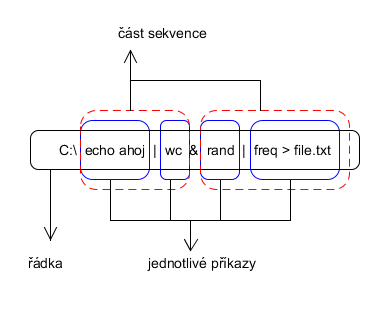
\includegraphics[width=0.75\textwidth]{./command.png}
\caption{Parsování příkazů}
\end{figure*}

\subsection{Parser}
Zpracování vstupu se provádí v souboru \verb+c_cmd.cpp+.
Řádka je nejprve rozdělena na sekvenční části, které odděluje znak \verb+;+. Sekveční části se pak parsují podle rour na jednotlivé příkazy. Ze samotných příkazů se pak získá název příkazu, parametry a přesměrování.



\subsection{Roura}
Roura (\verb+pipe.h+) je implementována kruhovým bufferem. Jako synchronizační mechnanismus jsou použity dva semafory a jedna kritická sekce. Má dva handlery - jeden pro čtení, druhý pro zápis.

\subsection{Seznam příkazů}
Seznam implementovaných příkazů, které můžete zadávat do příkazové řádky:
\label{cmd}
\begin{itemize}
\item cmd, echo, cd, tree
\item dir, mkdir (md), rm (rd)
\item freq, rand, type
\item scan, který vypisuje ascii hodnotu ze vstupu
\item pipe, který vypisuje vstup na výstup
\item info, který vypíše parametry
\item exit ukončí cmd proces

Lze zadávat sekvence příkazů oddělené \verb+;+ v rámci jednoho vstupního řádku. Příkazy lze také přesměrovávat a spojovat.
\end{itemize}

\subsection{Spouštění příkazů}

Hlavní proces cmd čte vstup, který parsuje. Pokud narazí na středník nebo novou řádku přestane parsovat vstup a zpracuje příkaz. Příkaz se parsuje podle rour. Za každý znak roury se vytvoří nová roura. První příkaz pak dostane vstup od cmd a poslední příkaz předá výstup a chybové hlašení zpátky cmd. Následně se příkazy spojí pomocí rour. Po spojení se všechny příkazy spustí a čeká se na poslední příkaz. Až doběhne předá se řízení cmd, který čte opět vstup.


\begin{figure*}[!h] 
\centering
 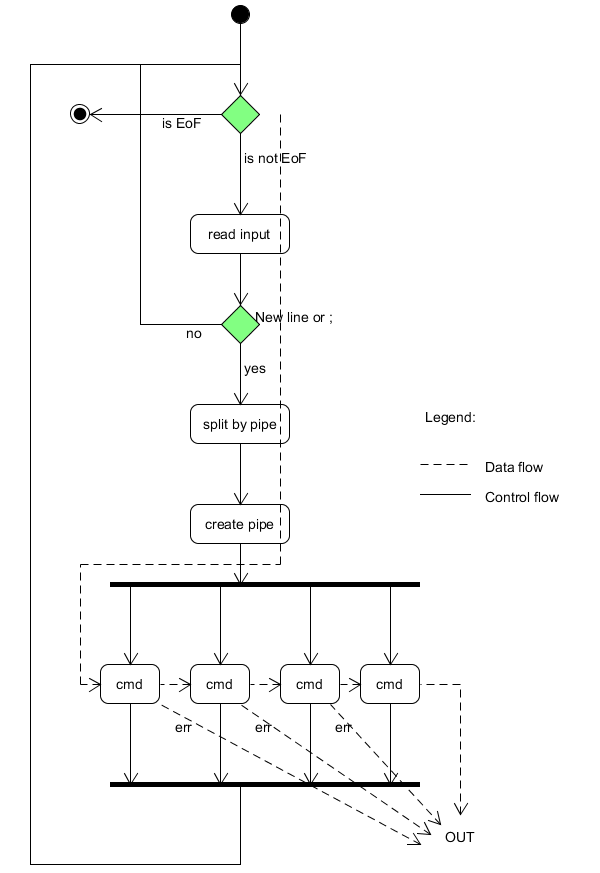
\includegraphics[width=1\textwidth]{./flow2.png}
\caption{Data a control flow diagram}
\end{figure*}


\section{Uživatelská příručka}
Pro spuštění programu stačí otevřít spustitelný soubor \emph{os.exe}. V terminálovém okně se zobrazí aktuální adresář, ve kterém se nacházíte. V tuto chvíli můžete zadávat dostupné příkazy (viz \ref{cmd}).


Každý příkaz může být přesměrován na výstup zápisem  \verb+příkaz > soubor+ a na vstup  \verb+příkaz< soubor+. Lze i přesměrovat na konec souboru konstrukcí \textgreater\textgreater. Příkazy je dále možné spojovat pomocí rour pro nasměrování výstupu jednoho procesu na vstup následujícího procesu  \verb+příkaz1 | příkaz2+.

Ukončení čtení se provádí CTRL+Z. 
V spuštěné příkazové řádce lze spustit další příkazovou řádku. Každá příkazová řádka se ukončuje příkazem \verb+exit+. 



\section{Závěr}

V rámci této práce jsme implementovali zadané příkazy, roury a přesměrování a splnili jsme tak všechny body zadání. Snažili jsme se vyvarovat zmíněným častým chybám a dbali jsme na doporučení uvedená na CW - spuštění shellu z shellu atp. Nad rámec zadání jsme umožnili přesměrování chybového výstupu a také jsme implementovali příkaz scan, který vypisuje ASCII hodnoty znaků ze vstupu na výstup.

Aplikaci jsme během vývoje průběžně testovali, a díky tomu se nám podařilo odstranit velké množství chyb. U většiny příkazů jsme neimplementovali jejich parametry, ale v rámci rozšíření práce by bylo možné tuto funkcionalitu dodělat.
Díky této semestrální práci jsme si osvěžili práci s pamětí, ukazateli a vlákny, avšak hlavním přínosem bylo hlubší pochopení toho, jak vlastně shell funguje.





\end{document}
